\documentclass[10pt,twocolumn]{article}
\usepackage[letterpaper,margin=0.68in]{geometry}
\usepackage{amsmath,amssymb,booktabs,graphicx,array,multirow,enumitem,float}
\graphicspath{{../}{./}}
\usepackage[hidelinks]{hyperref}
\setlength{\parindent}{1em}
\setlist[itemize]{leftmargin=1.35em,itemsep=0.15em,topsep=0.15em}
\renewcommand{\arraystretch}{1.12}
\setlength{\belowcaptionskip}{4pt}
\title{\vspace{-1.2em}\textbf{Interpretable Adaptive Kernel Banks for Cancer Classification with Limited Data}}
\author{Masoud Vahid Dastgerdi\\ \textit{Higher School of Economics}\\ \texttt{masoud.vahid10@gmail.com}
\and Oleg Stanislavovich Pianykh\\ \textit{Massachusetts General Hospital}\\ \texttt{opianykh@mgh.harvard.edu}}
\date{}
\begin{document}
\maketitle

\begin{abstract}
Cancer classification from annotated medical images is difficult when training data are limited. High-capacity convolutional neural networks (CNNs) can be accurate, but they require substantial supervision and give little insight into the visual evidence behind a decision. We propose an interpretable alternative built from a small bank of jointly learned circularly symmetric kernels. Each image region is summarized by pooled responses of the learned kernels, and kernels whose responses on training images are nearly collinear are identified by correlation, clustered, sign-aligned, and merged. The resulting classifier is defined by a handful of one-dimensional radial profiles rather than an opaque filter stack. We evaluate the approach with patient-level splits on a breast cohort of high-resolution annotated images and a lower-grade glioma (LGG) MRI cohort. On breast images, merging reduces a 16-kernel bank to nine kernels with no loss in held-out discrimination, and the merged bank outperforms analytic selected-kernel banks that use ten times as many kernels, reaching 0.94 test ROC-AUC against 0.96 for a CNN reference. On MRI, the learned bank improves substantially over a single radial kernel. A controlled sweep over bank size shows that on breast images much of the gain over a single kernel comes from the pooled response encoding, whereas on MRI retaining several distinct kernels matters more. The method therefore offers a compact, inspectable representation for limited-data cancer classification, with an explicit account of where its capacity resides.
\end{abstract}

\section{Introduction}
Medical-image classifiers can support cancer detection, lesion triage, and localization. Their use is especially challenging in limited-data settings, where the number of annotated cases may be too small to reliably train a high-capacity model and where an inspectable account of image evidence is valuable. CNNs have become dominant because they learn useful visual representations directly from data \cite{krizhevsky2012,litjens2017}. Their performance, however, is commonly obtained with representations that are difficult to interpret and with data demands that can be impractical for specialized clinical cohorts.

Before end-to-end deep learning, medical-image analysis commonly used explicit visual descriptors: edge, blob, texture, and co-occurrence features \cite{haralick1973,kass1988,haralick1979}. Gaussian derivatives and difference-of-Gaussians describe smoothing, boundaries, and local contrast \cite{lowe2004}; Gabor filters capture oriented texture \cite{daugman1985}; and histogram-of-oriented-gradients and local binary patterns describe local gradients and intensity relationships \cite{dalal2005,ojala2002}. Such representations remain useful in small-data cancer studies, including breast histopathology, mammography, cervical histopathology, and thyroid cytology \cite{doyle2008,ojansivu2013,gopinath2013,zheng2010,kadhim2023,he2023}. Yet prior handcrafted pipelines generally fix a descriptor family in advance. They do not jointly adapt a compact, interpretable kernel set to the data, nor do they explicitly reduce redundancy after learning.

Hybrid approaches offer a useful middle ground: constrained visual features remain inspectable while a lightweight classifier learns the decision boundary. Recent work has combined texture and deep features for renal cancer detection \cite{cai2022}, and feed-forward breast-image classifiers have used logistic-regression or SVM modules \cite{karuppasamy2024}. Sparse selection \cite{zhu2020} and maximal marginal relevance (MMR) \cite{carbonell1998} can also produce compact feature sets. The outstanding gap is a method that is both adapted to a limited medical dataset and transparent at the level of its learned visual primitives.

We address this gap with a learned radial-kernel bank. Circular symmetry constrains each kernel to a one-dimensional radial profile, reducing its degrees of freedom and making its form directly inspectable. The approach learns several profiles jointly, summarizes their responses with a small interpretable readout, and then merges kernels that are redundant on real training images. The objective is not to replace CNNs universally, but to determine how much discriminative performance can be retained with a compact representation under constrained supervision, and to identify where the capacity of such a model actually resides.

The contributions are:
\begin{itemize}
\item a limited-data cancer-classification framework based on jointly learned, circularly symmetric kernels and a lightweight classifier;
\item response-space redundancy merging, in which kernels are clustered by real-image response correlation, sign-aligned, and merged into the smallest bank that preserves validation quality;
\item an ablation separating the value of multiple kernels from that of the pooled-response encoding, evaluated on breast and LGG MRI cohorts using patient-level splits; and
\item comparison with analytic selected-kernel models, sparse selection, composite and rotation-invariant variants, and a CNN reference.
\end{itemize}

\section{Methods}
\subsection{Problem formulation}
Let $x\in\mathbb{R}^{H\times W}$ denote an image region with binary label $y\in\{0,1\}$, where positive regions are sampled from a malignant or tumor annotation and negative regions from non-lesion tissue. Given $\mathcal{D}=\{(x_i,y_i)\}_{i=1}^N$, the task is to estimate $p(y=1\mid x)$. Every model considered here shares one structure: a bank of convolution kernels $\{k_j\}_{j=1}^{K}$ maps a region to response maps $z_j=x*k_j$, each map is reduced to a few pooled scalars, and a lightweight classifier operates on the concatenated feature vector $\phi(x)$. The models differ in how the kernels are obtained, analytic families versus learned radial profiles, in how many are retained, and in how each response map is summarized. Because the classifier is linear or nearly so, the kernels and their pooled summaries are the only place where visual evidence enters the decision, which is what makes the representation inspectable.

\subsection{Data and preprocessing}
The breast cohort contains high-resolution TIFF images of approximately $6000\times4750$ pixels with expert red-contour malignant annotations: 127 malignant images, 365 normal images, and 125 annotation files. Contours are converted to binary lesion masks by thresholding the red channel while suppressing green and blue, followed by morphological dilation, erosion, closing, and hole filling. We extract $128\times128$-pixel image regions at native resolution. Positive regions require at least 0.80 lesion coverage and negatives at most 0.02; negatives are drawn both near and far from the lesion. Regions with a low fraction of nonzero intensity are excluded as low-tissue.

The LGG MRI cohort of Buda et al. \cite{buda2019}, derived from The Cancer Genome Atlas and The Cancer Imaging Archive (TCGA/TCIA), comprises fluid-attenuated inversion recovery (FLAIR) slices with manual tumor masks from 110 patients. From the masks we sample $64\times64$-pixel regions: positives have at least 0.80 tumor coverage, while negatives have zero coverage, with a subset drawn from a dilated band around the tumor so that the negative class contains hard near-boundary examples. A tissue-occupancy requirement removes background-air regions, and per-class caps balance the two classes.

Patient or image identifiers, inferred from filenames, determine fixed 70/15/15 train/validation/test splits, so no source image contributes to more than one split (Table~\ref{tab:datasets}). The slight imbalance in the breast splits follows from patient-level assignment and region-extraction yield. Regions are loaded in grayscale. Breast regions are not intensity-standardized because absolute contrast is informative in that cohort; MRI regions are standardized per region because scanner-dependent offsets carry no diagnostic meaning. Section~\ref{sec:results-std} quantifies the cost of reversing this choice.

\begin{table}[!t]
\centering
\caption{Image-region counts. Splits are assigned at patient/image level.}
\label{tab:datasets}
\footnotesize
\begin{tabular}{llrrr}
\toprule
Cohort & Split & Pos. & Neg. & Total\\
\midrule
\multirow{4}{*}{Breast} & Train & 2,900 & 3,430 & 6,330\\
 & Validation & 1,080 & 790 & 1,870\\
 & Test & 1,040 & 830 & 1,870\\
 & Total & 5,020 & 5,050 & 10,070\\
\midrule
\multirow{4}{*}{Brain LGG} & Train & 3,000 & 3,000 & 6,000\\
 & Validation & 1,000 & 1,000 & 2,000\\
 & Test & 1,000 & 1,000 & 2,000\\
 & Total & 5,000 & 5,000 & 10,000\\
\bottomrule
\end{tabular}
\end{table}

\subsection{Learned radial bank and encoding}

The primary model replaces an unconstrained $s\times s$ kernel with a circularly symmetric one. Let $B_r\in\{0,1\}^{s\times s}$ be the indicator of the shell of pixels at integer distance $r$ from the kernel center. A radial kernel is
\begin{equation}
k=\sum_{r=0}^{R}f(r)\,B_r,
\label{eq:radial}
\end{equation}
where $f(r)$ is a learned one-dimensional profile, so an $s\times s$ filter is described by $R+1$ numbers. The constraint reduces the degrees of freedom, imposes an isotropic bias suited to blob-like and halo-like tissue patterns, and makes every kernel readable as a single curve. Shells beyond a radius $R_{\max}$ stay fixed at their seed values, which bounds the effective support.

We learn $K=16$ profiles jointly. Profiles are seeded from two sources chosen to span different spatial scales: variants of the rotation-invariant profile extracted from the composite kernel of Section~\ref{sec:baselines}, and synthetic center--surround shapes of increasing width. Training minimizes a class-balanced binary cross-entropy through a 32-unit hidden head with dropout 0.1, regularized by
\begin{equation}
\begin{aligned}
\mathcal{L}={}&\mathcal{L}_{\rm cls}+\lambda_s\mathcal{L}_{\rm smooth}+\lambda_c\mathcal{L}_{\rm curv}\\
&+\lambda_a\mathcal{L}_{\rm anchor}+\lambda_n\mathcal{L}_{\rm scale}+\lambda_d\mathcal{L}_{\rm div}.
\end{aligned}
\label{eq:objective}
\end{equation}
The smoothness and curvature terms in Eq.~\eqref{eq:objective} penalize first and second differences of $f$ along $r$; the anchor term limits drift from the seed; the scale term keeps profile norms comparable; and $\mathcal{L}_{\rm div}=\operatorname{mean}_{i\neq j}\exp(-\lVert f_i-f_j\rVert^2)$ discourages profiles from collapsing onto one another. The checkpoint with the highest validation ROC-AUC is retained, and a class-balanced logistic model is then refit on the frozen bank to provide calibrated probabilities.

A single scalar per kernel discards most of the response map. Each kernel therefore contributes three pooled statistics of $z=x*k_j$:
\begin{equation}
\psi_j(x)=\Big[\operatorname{mean}|z|,\ \max|z|,\ \tfrac{1}{m}\!\sum_{\text{top-}m}\! z-\tfrac{1}{m}\!\sum_{\text{top-}m}\!(-z)\Big],
\label{eq:encoding}
\end{equation}
where the top-$m$ sums run over the $m$ largest entries of $z$ and of $-z$, and $m$ is a fixed fraction of the map (1\% for breast regions and 10\% for the smaller MRI regions). The three statistics answer different questions. Mean magnitude measures how much of the region responds, which separates diffuse texture from a quiet background. Maximum magnitude measures the strongest single structure, which detects a focal pattern even when the rest of the region is quiet. The two are decoupled in practice: a small lesion in a large region gives a high maximum with a low mean, whereas widespread texture gives the opposite, so neither can be recovered from the other. The signed statistic distinguishes bright-on-dark from dark-on-bright structure, which both absolute statistics conflate. A bank of $K$ kernels thus yields $3K$ features. Section~\ref{sec:results-sweep} quantifies how much of the method's gain comes from this encoding rather than from kernel count.

\subsection{Redundancy merging}
\label{sec:merge}
Jointly trained profiles need not be independent. Two profiles that look different can still produce nearly the same responses on real tissue, and a profile and its sign-reversed copy carry identical information after pooling. The bank is therefore compressed after training, using the geometry of the responses rather than the geometry of the kernels.

Let $r_j\in\mathbb{R}^{n}$ collect the centered convolutional responses of kernel $j$ over the pixels of a fixed subsample of training regions. The classifier only ever observes functions of these vectors, so what matters is the subspace they span. If $|\rho_{ij}|\approx1$, where $\rho_{ij}$ is the Pearson correlation of $r_i$ and $r_j$, the two vectors are nearly collinear: replacing the pair by a single kernel leaves the span, and hence the set of achievable decision functions, essentially unchanged. If $\rho_{ij}=0$ the vectors are orthogonal and the two kernels supply complementary evidence. Orthogonality in kernel space is not a substitute for this test. Natural image statistics are strongly correlated across scales and orientations, so two kernels with orthogonal weights routinely produce correlated responses on tissue, and only the response-space test reflects what the classifier can use. The redundancy of a pair is accordingly measured by the distance
\begin{equation}
d_{ij}=1-|\rho_{ij}|,
\label{eq:distance}
\end{equation}
where the absolute value makes a sign-reversed pair maximally redundant.

Rather than assuming that the initial count $K$ is necessary, we start from the full $K$-kernel bank and ask whether a $(K-1)$-kernel bank spans the same evidence, then a $(K-2)$-kernel bank, and so on down to a single kernel. Average-linkage hierarchical clustering on Eq.~\eqref{eq:distance} provides exactly this nested sequence: cutting the dendrogram at $K'$ clusters gives the $K'$-kernel bank. Each cluster is collapsed to one profile: members are sign-aligned to the cluster medoid, averaged, and renormalized to the members' mean norm. Because averaging acts on the radial coefficients $f(r)$ and the result is re-expanded through Eq.~\eqref{eq:radial}, every merged kernel remains exactly radial and inspectable. For each $K'$ the same class-balanced logistic head is refit on the reduced bank, and we retain the smallest $K'$ whose validation ROC-AUC and validation threshold-tuned accuracy both remain within a tolerance $\tau$ of the full bank. All selection uses validation data only; test data are touched only for final reporting.

\subsection{Baselines and experimental protocol}
\label{sec:baselines}
\paragraph{Analytic kernel banks.} The analytic comparison models draw kernels from nine families: Gaussian, anisotropic Gaussian, difference-of-Gaussians, Laplacian-of-Gaussian, Gabor, derivative, two-point co-occurrence, center--neighbor local-contrast, and discrete-Laplacian filters. Family parameters are sampled either independently at random or with Sobol quasi-Monte Carlo (QMC) sequences, which cover heterogeneous parameter spaces more evenly. Each analytic kernel is summarized by the single scalar
\begin{equation}
r_j(x)=\max_{u,v}\left|(x*k_j)_{u,v}\right|.
\label{eq:response}
\end{equation}
Candidates are ranked by the univariate ROC-AUC and Fisher score of $r_j$ on training regions, and MMR then selects a subset that is discriminative and nonredundant:
\begin{equation}
k^*=\arg\max_{k_j\notin S}\Big[\lambda\,\mathrm{AUC}(k_j)-(1-\lambda)\max_{k_\ell\in S}\left|\rho(r_j,r_\ell)\right|\Big],
\label{eq:mmr}
\end{equation}
where $S$ is the current selection and $\lambda=0.75$. The redundancy term in Eq.~\eqref{eq:mmr} uses the same response correlation as Eq.~\eqref{eq:distance}, so selection and merging are two applications of one principle: MMR avoids adding a collinear kernel, and merging removes one after learning. A logistic classifier is trained on the selected responses.

\paragraph{Derived analytic models.} Composite kernels compress a selected bank by grouping its kernels and summing each group with normalized weights, $k_{\rm comp}=\sum_i w_i k_i$, so that eight composites, or a single composite, replace the selected kernels. Rotation-averaged kernels enforce right-angle invariance by averaging a composite over its four rotations, $k_{\rm RI}=\tfrac14\sum_{q=0}^{3}\operatorname{rot}_{90q}(k_{\rm comp})$; a finer variant averages every $10^\circ$. Adaptive best-subset selection (ABESS) \cite{zhu2020} provides a sparse-selection alternative to MMR under an $\ell_0$ objective. A shape-sensitive bank of triangular and square kernels tests non-circular primitives.

\paragraph{CNN reference.} The reference network takes $128\times128$ RGB breast regions through four convolutional blocks with batch normalization, ReLU, max pooling, and dropout, followed by adaptive average pooling and a two-layer linear head. It is trained with cross-entropy and AdamW at learning rate $3\times10^{-4}$, weight decay $10^{-4}$, patience six, and at most 25 epochs; the best model by validation ROC-AUC occurred at epoch six. The CNN was evaluated on the breast cohort only.

\paragraph{Evaluation protocol.} The primary metric is the area under the receiver operating characteristic curve (ROC-AUC), which is threshold independent and remains informative under the modest breast-class imbalance. Accuracy is reported at the default 0.5 threshold for the cross-model comparison in Table~\ref{tab:main-results}, and at a threshold tuned on validation data for the radial-bank analyses in Tables~\ref{tab:minimal-bank} and \ref{tab:sweep}; for the radial banks the two conventions differ by less than 0.001. CNN experiments additionally record precision, recall, F1, loss, and confusion matrices. All model selection, including checkpoint choice, threshold tuning, and the merged-bank size, uses validation data; test data are used only for final reporting.

\paragraph{Implementation details.} The radial bank uses $K=16$ seeds, three statistics per kernel, Adam, and batch size 128 on both cohorts. The breast configuration uses $31\times31$ kernels, $R_{\max}=20$, 25 epochs, and profile learning rate $2\times10^{-3}$ chosen on validation ROC-AUC from $\{10^{-2},2\times10^{-3},5\times10^{-4}\}$. The MRI configuration uses $63\times63$ kernels, $R_{\max}=30$, 40 epochs, and profile learning rate $10^{-2}$. Merging uses $\tau=0.005$. Analytic banks use $31\times31$ kernels, 60 epochs, batch size 64, and learning rate $5\times10^{-4}$; the strongest configurations select 90 kernels from pools of up to 4,500 candidates, and compact models with one, three, and five kernels are also reported.

The analytic and learned-radial experiments answer complementary questions. Analytic banks test whether a broad library of known visual patterns, selected after response ranking, is sufficient. The learned bank tests whether a strongly constrained representation can adapt to the cohort without becoming an unconstrained CNN. Composite and rotation-averaged models evaluate two ways of simplifying selected filters, and ABESS evaluates sparse selection under a different objective. These variants therefore compare representation and compression strategies; they are not interchangeable estimates of one model's uncertainty.

\section{Results}
\subsection{Primary comparison}
Table~\ref{tab:main-results} reports held-out breast results for all model families. The nine kernel merged radial bank has the highest test ROC-AUC among the interpretable models and exceeds every analytic selected bank, including the 90 and 200 kernel configurations, while using at most one tenth as many kernels. Its validation and test values are close, as are those of the unmerged 16 kernel bank. The CNN reference has the highest test ROC-AUC and accuracy overall, with a margin of 0.021 ROC-AUC over the merged bank. Among the analytic banks, test ROC-AUC varies within a narrow range whereas accuracy varies more widely; the ABESS bank shows the largest gap between the two metrics.

\begin{table*}[!t]
\centering
\caption{Held-out breast results. Accuracy is at the default 0.5 threshold. ``Kernels'' is the number of retained kernels; the CNN learns its filters end to end.}
\label{tab:main-results}
\small
\begin{tabular}{p{0.40\linewidth}ccccc}
\toprule
Model / configuration & Kernels & Val AUC & Val Acc. & Test AUC & Test Acc.\\
\midrule
\textbf{Minimal merged radial bank} & \textbf{9} & \textbf{0.9373} & \textbf{0.8856} & \textbf{0.9415} & \textbf{0.8727}\\
Radial kernel bank before merging & 16 & 0.9388 & 0.8861 & 0.9411 & 0.8754\\
Learned single radial kernel & 1 & 0.9189 & 0.8545 & 0.9286 & 0.8668\\
CNN reference & -- & 0.9445 & 0.8818 & \textbf{0.9626} & \textbf{0.9021}\\
Selected kernel bank with QMC sampling & 90 & 0.9270 & 0.8603 & 0.9387 & 0.8866\\
Selected kernel bank, variant A & 90 & 0.9271 & 0.8636 & 0.9377 & 0.8882\\
Selected kernel bank, variant B & 90 & 0.9273 & 0.8620 & 0.9376 & 0.8888\\
Larger selected kernel bank & 200 & 0.9159 & 0.8514 & 0.9313 & 0.8578\\
Sparse ABESS-selected bank & 200 & 0.9095 & 0.7849 & 0.9236 & 0.7690\\
Shape-sensitive triangular/square bank & 24 & 0.9109 & 0.8481 & 0.9221 & 0.8465\\
\bottomrule
\end{tabular}
\end{table*}

\subsection{Radial banks and merging}

On both cohorts the 16 kernel bank outperforms the corresponding single learned radial kernel (Table~\ref{tab:minimal-bank}). The breast single-kernel reference is the strongest saved single radial run under the same radial support $R_{\max}=20$ as the bank, a monotone-decreasing variant; across all radial supports the best single kernel reaches 0.9227 test ROC-AUC, so the comparison is insensitive to this choice. Constrained single-kernel variants trade accuracy for interpretability: an unconstrained learned radial kernel reaches 0.9286 test ROC-AUC (Table~\ref{tab:main-results}), whereas a signed compact variant with a hard radial cutoff and decay regularization drops to 0.8808, and an independently initialized smooth signed variant reaches 0.9187.

On breast images, the merging procedure of Section~\ref{sec:merge} reduces 16 profiles to nine, a 44\% reduction, and leaves test ROC-AUC and accuracy unchanged within 0.002. The merge grouped the trained bank into one cluster of six profiles, two pairs, and six singletons, so most of the reduction came from a single family of near duplicate profiles. On MRI the 16-kernel bank improves test ROC-AUC over a single kernel by 0.072, a larger relative gain than on breast data. The validation selected nine kernel MRI bank, which has the same cluster structure of one six member cluster, two pairs, and six singletons, satisfies the validation tolerance but loses 0.029 test ROC-AUC relative to the full bank; intermediate sizes lose less, with the eight kernel bank retaining 0.7434 (Table~\ref{tab:sweep}).

\begin{table*}[!t]
\centering
\caption{Radial banks and single radial kernels. ``Features'' is the number of scalars seen by the classifier. Merged banks are selected on validation data with $\tau=0.005$; accuracy uses the validation-tuned threshold.}
\label{tab:minimal-bank}
\small
\begin{tabular}{llccccc}
\toprule
Cohort & Model & Kernels & Features & Val AUC & Test AUC & Test Acc.\\
\midrule
\multirow{3}{*}{Breast} & Best single learned radial kernel & 1 & 1 & 0.9100 & 0.9212 & 0.8412\\
 & Radial kernel bank & 16 & 48 & \textbf{0.9388} & 0.9411 & \textbf{0.8749}\\
 & \textbf{Minimal merged bank} & \textbf{9} & \textbf{27} & 0.9373 & \textbf{0.9415} & 0.8733\\
\midrule
\multirow{3}{*}{Brain LGG} & Single learned radial kernel & 1 & 3 & 0.7281 & 0.6903 & 0.6365\\
 & Radial kernel bank & 16 & 48 & \textbf{0.7849} & \textbf{0.7624} & \textbf{0.6750}\\
 & \textbf{Minimal merged bank} & \textbf{9} & \textbf{27} & 0.7801 & 0.7335 & 0.6640\\
\bottomrule
\end{tabular}
\end{table*}

\subsection{Kernel count versus encoding}
\label{sec:results-sweep}
Because the merge sweep refits the same head at every $K'$, it doubles as an ablation on kernel count with the encoding held fixed (Table~\ref{tab:sweep}). On breast images a bank merged all the way to one kernel still reaches 0.9346 test ROC-AUC, above the 0.9212 of the best directly optimized single radial kernel. The two models have the same number of filters. They differ only in that the merged model reads the three statistics of Eq.~\eqref{eq:encoding} and uses a class-balanced logistic head, whereas the single-kernel reference reads the one scalar of Eq.~\eqref{eq:response}. Of the total breast improvement from 0.9212 to 0.9415, 0.0134 is already present at $K'=1$ and the remaining 0.0069 comes from increasing $K'$ to nine. The optimization traces agree: on breast images the validation-selected checkpoint occurred at the first epoch for every profile learning rate tried, so the seeded profiles were already close to their final form. On MRI the picture reverses. Test ROC-AUC falls steadily as $K'$ decreases, apart from the dip at nine kernels, reaching 0.6671 at a single kernel, and the selected checkpoint occurred at epoch 33 of 40.

\begin{table}[!t]
\centering
\caption{Merge sweep. Each row refits the same class-balanced logistic head on a bank merged to $K'$ kernels. Asterisks mark validation-selected banks.}
\label{tab:sweep}
\footnotesize
\begin{tabular}{rcc@{\hskip 1.2em}cc}
\toprule
& \multicolumn{2}{c}{Breast} & \multicolumn{2}{c}{Brain LGG}\\
\cmidrule(lr){2-3}\cmidrule(lr){4-5}
$K'$ & Val AUC & Test AUC & Val AUC & Test AUC\\
\midrule
16 & 0.9389 & 0.9411 & 0.7850 & 0.7624\\
13 & 0.9388 & 0.9412 & 0.7740 & 0.7593\\
11 & 0.9364 & 0.9407 & 0.7755 & 0.7531\\
9$^*$ & 0.9373 & 0.9415 & 0.7801 & 0.7335\\
8 & 0.9365 & 0.9405 & 0.7794 & 0.7434\\
6 & 0.9299 & 0.9356 & 0.7593 & 0.7256\\
4 & 0.9295 & 0.9349 & 0.7220 & 0.7098\\
2 & 0.9259 & 0.9326 & 0.7039 & 0.6964\\
1 & 0.9271 & 0.9346 & 0.6218 & 0.6671\\
\bottomrule
\end{tabular}
\end{table}

\subsection{Intensity standardization}
\label{sec:results-std}
Applying per-region intensity standardization to the otherwise identical breast configuration reduces test ROC-AUC from 0.9411 to 0.8605 and accuracy from 0.8754 to 0.7898. This drop is larger than any gap between model variants in Table~\ref{tab:minimal-bank}.

\subsection{Analytic-bank comparisons}

Table~\ref{tab:compact} reports compact MMR models. A single selected kernel reaches 0.9157 test ROC-AUC and the best three-kernel model 0.9239, but thresholded accuracy ranges from 0.7594 to 0.8449 across configurations whose ROC-AUC differs by at most 0.014. Table~\ref{tab:sampling} compares kernel sampling and composition on matched 90-kernel banks. Sobol QMC sampling improves the base model over random sampling on both metrics, and the improvement carries over to the composite model. Composition itself loses information in every case: eight composites cost 0.034--0.045 test ROC-AUC relative to their base bank, and a single composite costs 0.074. Rotation averaging of a composite kernel yields identical metrics under $0^\circ$, $90^\circ$, $180^\circ$, and $270^\circ$ rotations of the test regions, at a cost of 0.018 ROC-AUC and 0.014 accuracy relative to the non-invariant composite on the same split; averaging every $10^\circ$ is slightly lower still. ABESS selection is competitive in ROC-AUC, 0.9236 with 200 features and 0.9216--0.9225 with three to five, but has lower accuracy than the corresponding MMR models in every reported run.

\begin{table*}[!t]
\centering
\caption{Compact MMR-selected analytic models on the breast cohort.}
\label{tab:compact}
\small
\begin{tabular}{p{0.40\linewidth}rrrrr}
\toprule
Compact configuration & Kernels & Val AUC & Val Acc. & Test AUC & Test Acc.\\
\midrule
Single-kernel selected model & 1 & 0.8994 & 0.8307 & 0.9157 & 0.8449\\
Single-kernel model from a larger candidate shortlist & 1 & 0.9010 & 0.8330 & 0.9179 & 0.8428\\
Three-kernel selected model, configuration A & 3 & 0.9085 & 0.8497 & 0.9101 & 0.8417\\
Three-kernel selected model, configuration B & 3 & 0.9085 & 0.8011 & 0.9239 & 0.7914\\
Five-kernel selected model & 5 & 0.9071 & 0.7765 & 0.9234 & 0.7594\\
\bottomrule
\end{tabular}
\end{table*}

\begin{table*}[!t]
\centering
\caption{Effect of kernel sampling and composition on 90-kernel selected banks (breast test set). Composite models replace the selected bank by eight composites unless noted.}
\label{tab:sampling}
\small
\begin{tabular}{lcccc}
\toprule
Configuration & Base AUC & Base Acc. & Composite AUC & Composite Acc.\\
\midrule
Random sampling & 0.9195 & 0.8646 & 0.8855 & 0.8063\\
Sobol QMC sampling & 0.9387 & 0.8866 & 0.8934 & 0.8176\\
Selected-bank variant B & 0.9376 & 0.8888 & 0.9026 & 0.8299\\
Single-composite compression & 0.9377 & -- & 0.8635 & 0.7797\\
\bottomrule
\end{tabular}
\end{table*}

\subsection{Qualitative outputs}
Figures~\ref{fig:confusion}--\ref{fig:minimal-bank-brain} provide diagnostic outputs: confusion matrices for the selected-kernel classifier and the CNN, and probability overlays from the merged radial bank on held-out images. Because the bank features are pooled statistics over a region rather than a single dense convolution, each overlay is produced by scoring a sliding grid of regions with exactly the classifier used at training time. The overlays allow inspection of whether high-probability areas correspond to lesion-like tissue, but no expert localization scoring or pixel-level localization metric is claimed.

\begin{figure}[H]
\centering
\begin{minipage}{0.48\linewidth}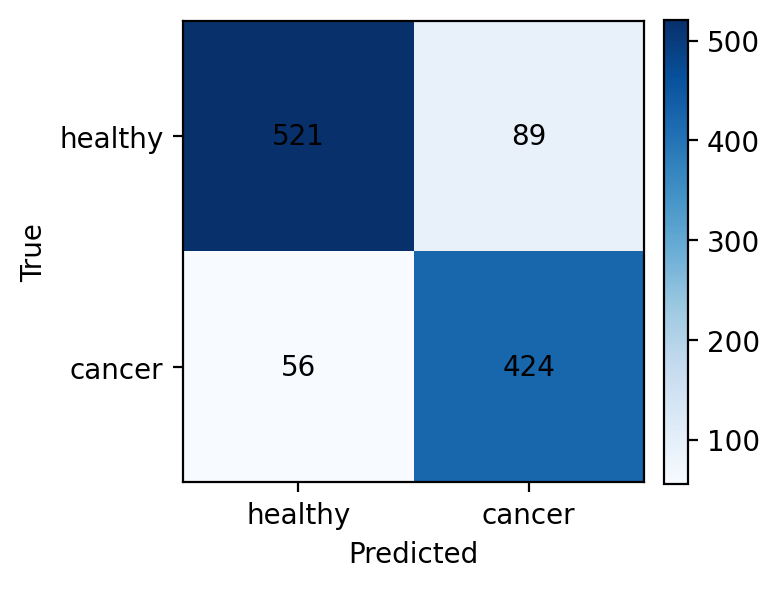
\includegraphics[width=\linewidth]{figures/selected_kernel_confusion.png}\end{minipage}\hfill
\begin{minipage}{0.48\linewidth}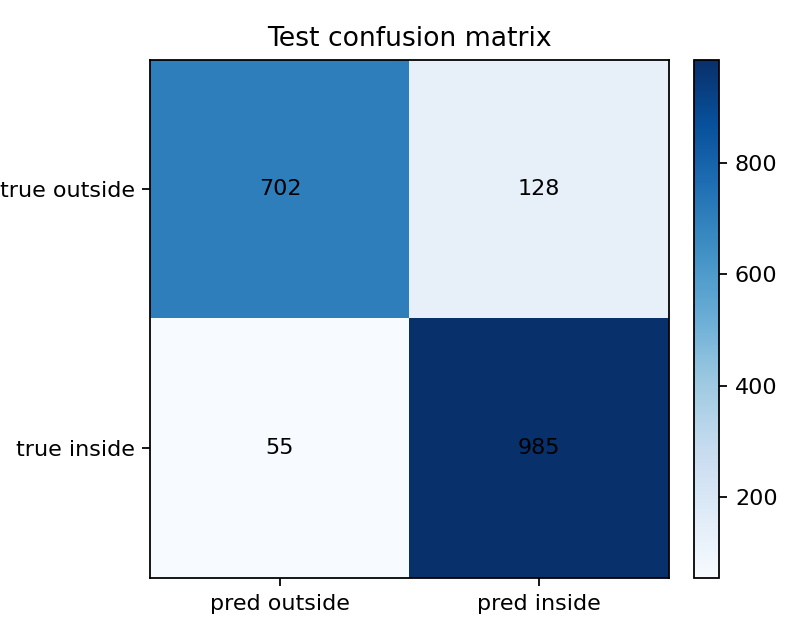
\includegraphics[width=\linewidth]{figures/cnn_confusion.png}\end{minipage}
\caption{Confusion matrices for the selected-kernel classifier (left) and CNN reference (right).}
\label{fig:confusion}
\end{figure}
\begin{figure}[H]
\centering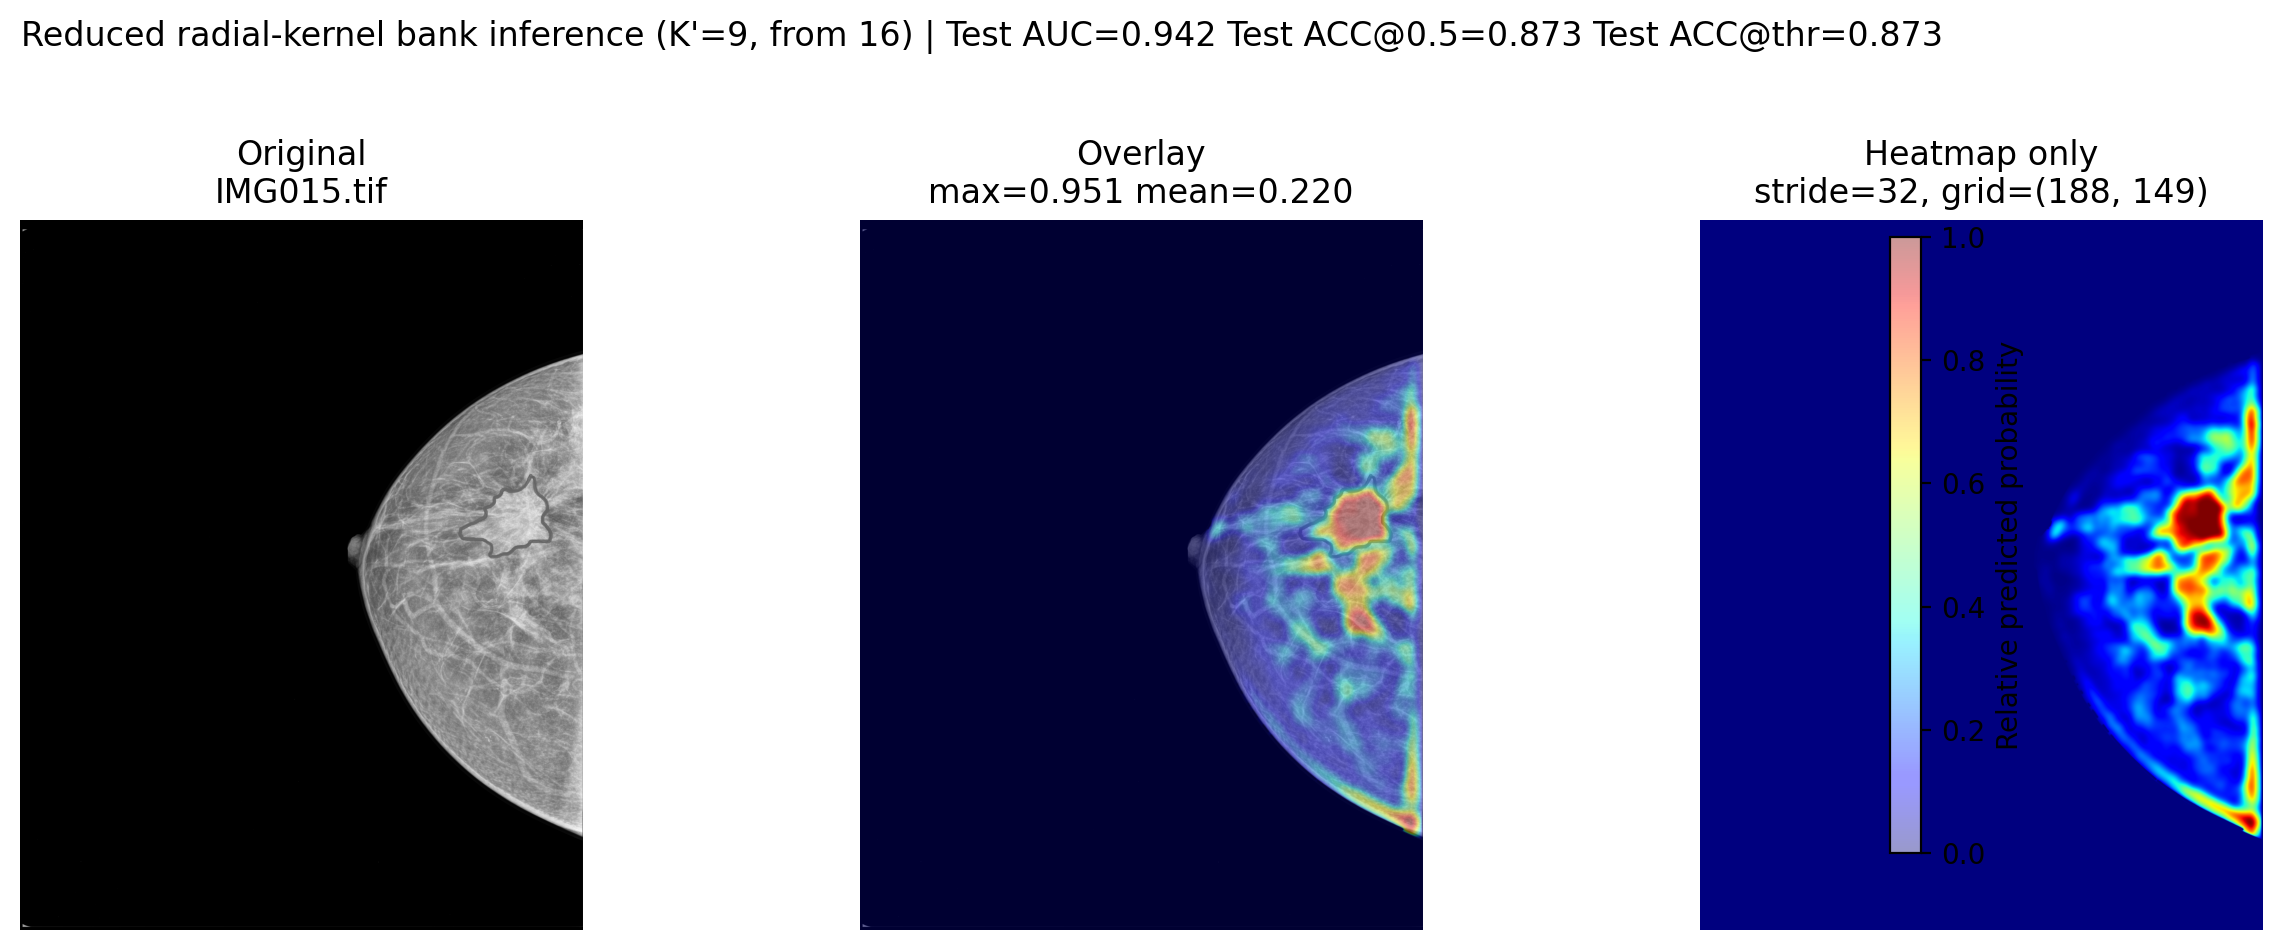
\includegraphics[width=\linewidth]{figures/minimal_bank_heatmap_breast.png}
\caption{Held-out breast-image probability overlay from the minimal merged radial bank.}
\label{fig:minimal-bank-breast}
\end{figure}
\begin{figure}[t]
\centering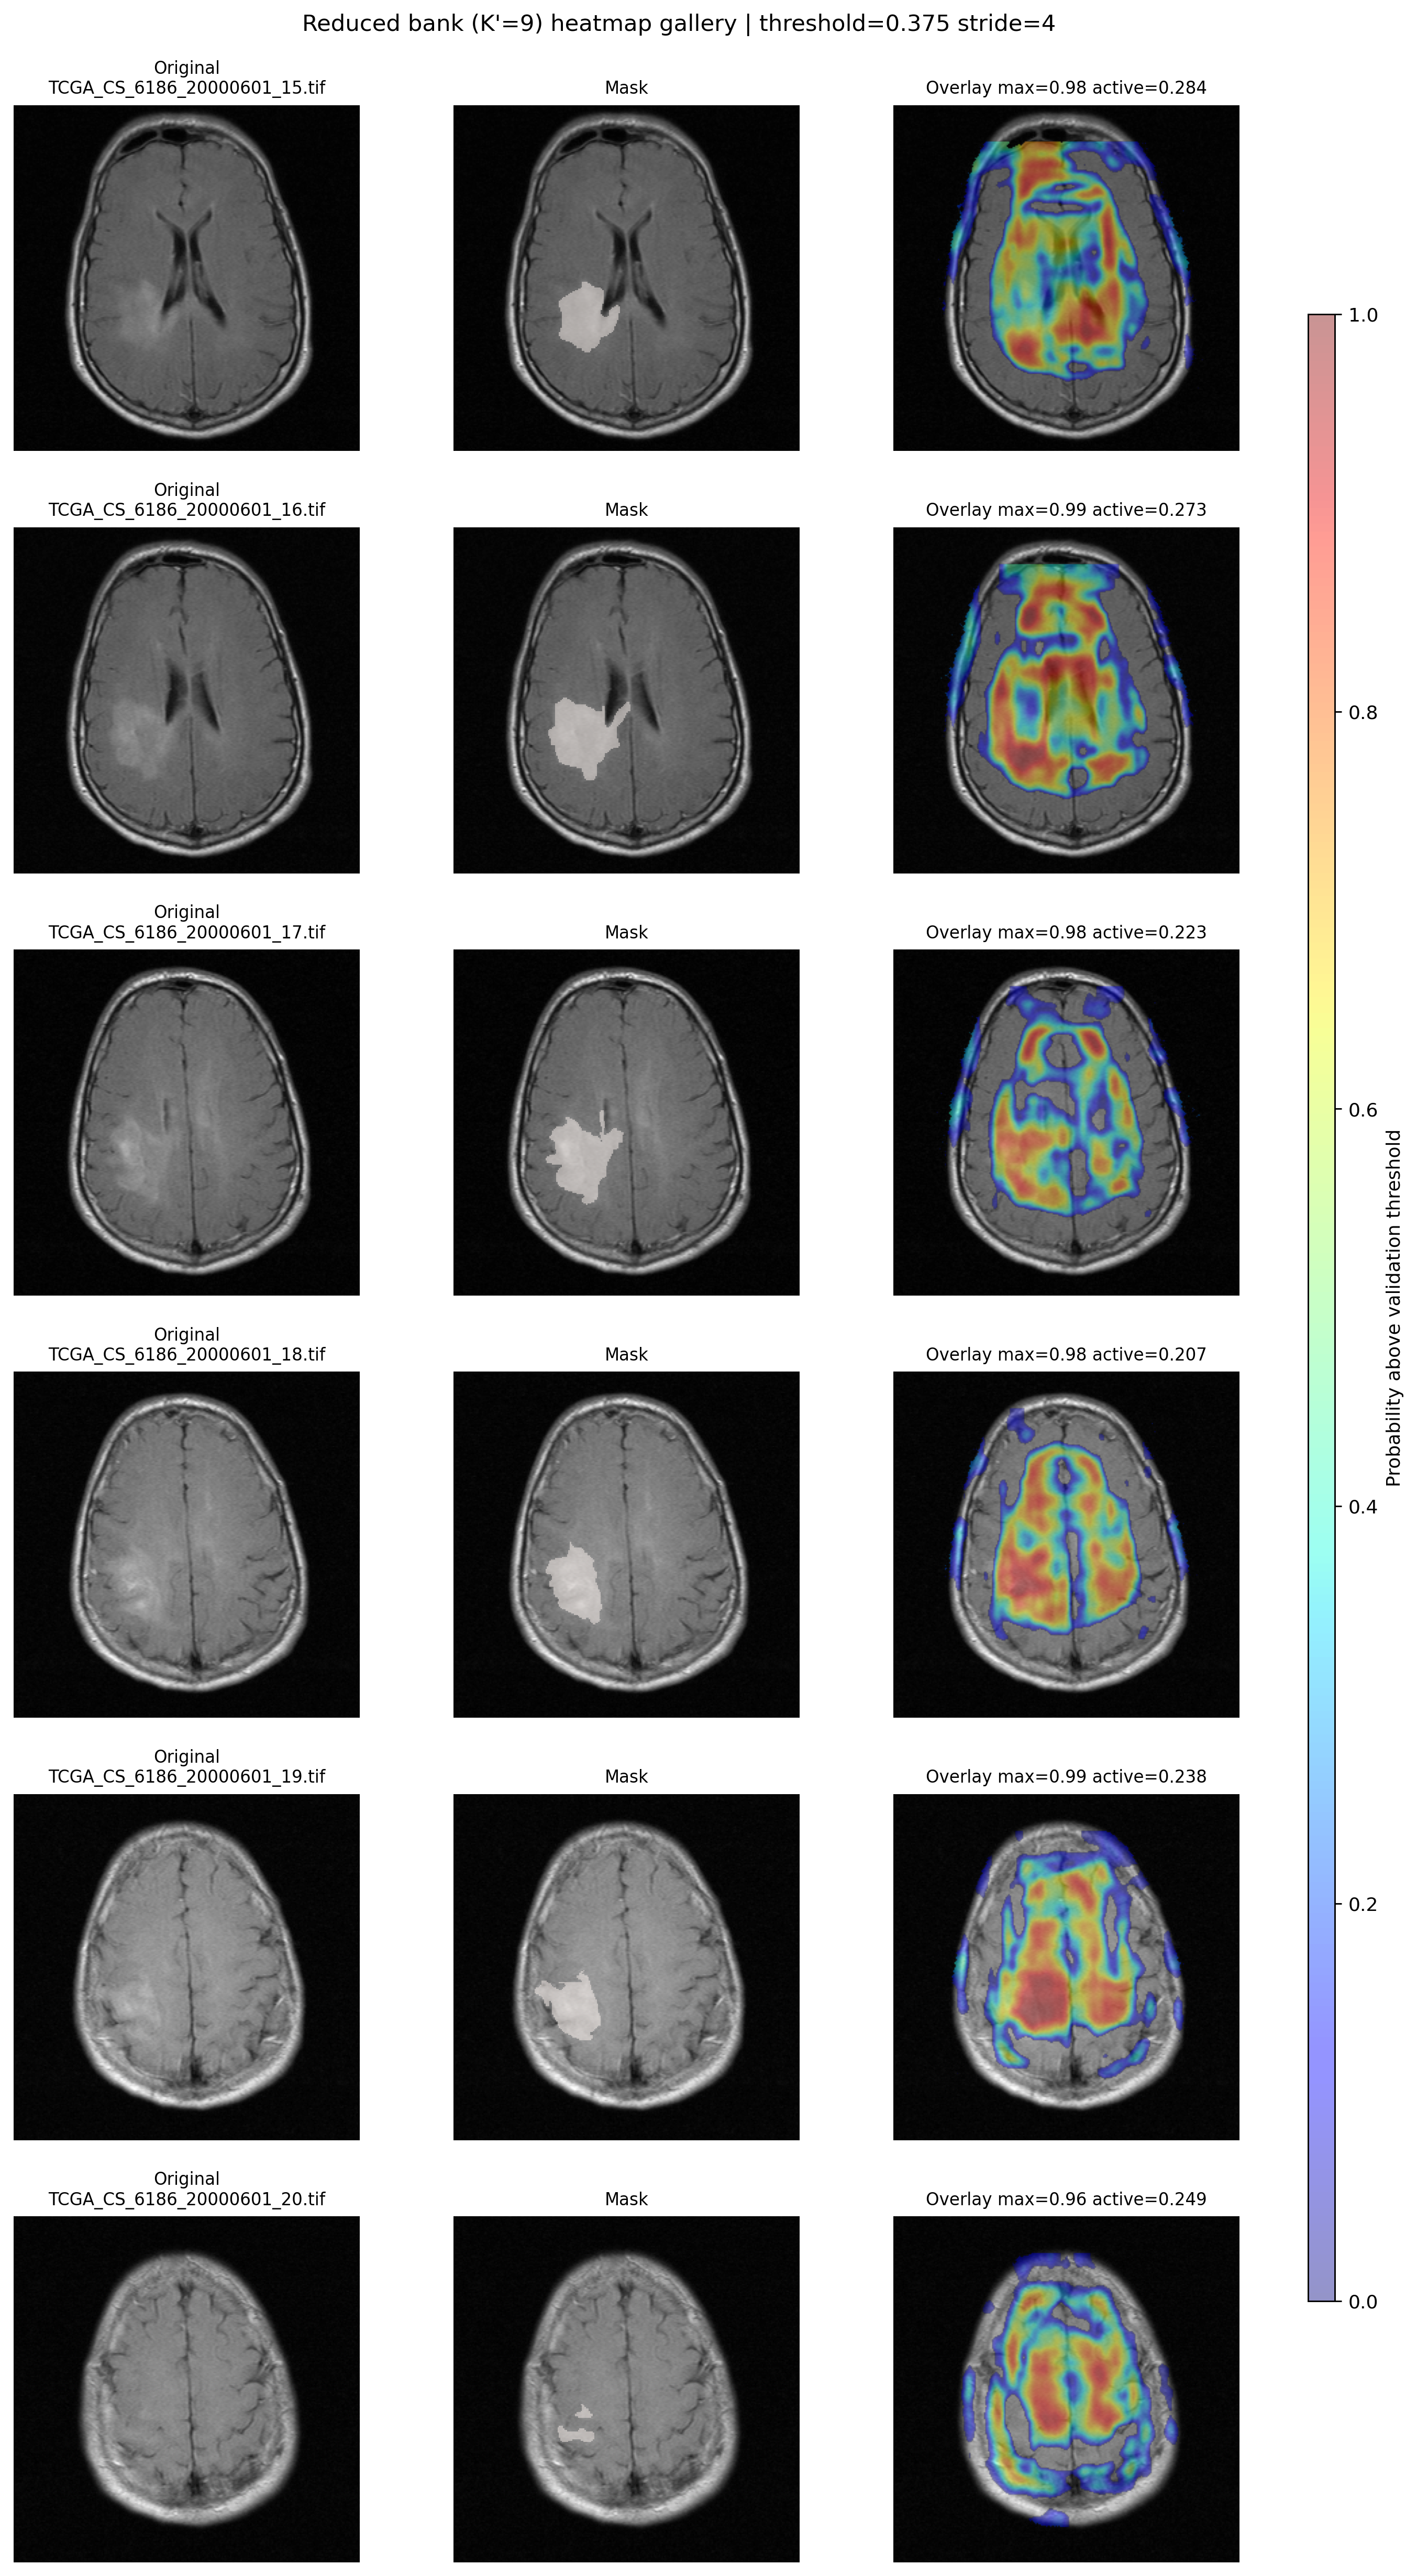
\includegraphics[width=0.56\linewidth]{figures/minimal_bank_heatmap_brain.png}
\caption{Held-out LGG MRI slices: image, tumor mask, and minimal-bank probability overlay.}
\label{fig:minimal-bank-brain}
\end{figure}

\section{Discussion and Conclusion}
This study investigates whether an interpretable model can accurately classify cancer when only limited training data are available. On the available cohorts the objective was met. A bank of jointly learned radial profiles, merged in response space, reaches held out discrimination that exceeds analytic selected kernel banks with ten times as many filters, and it does so with nine one-dimensional curves that can be inspected directly. On MRI the same procedure shows that several distinct radial patterns are needed and that the bank captures them. These outcomes correspond to the first two contributions: a limited data framework built on constrained learned kernels, and a merging procedure that obtains compactness by removing evidence-equivalent kernels rather than by fixing a small bank in advance.

The ablation, the third contribution, changes how the headline results should be read. On breast images a bank merged to a single kernel still beats the directly optimized single kernel, so most of the improvement comes from reading three complementary statistics from each kernel and calibrating with a class balanced head, not from having many filters. The first epoch checkpoints point the same way: the seeded profiles were already adequate, and a richer readout, not longer profile training, was the effective lever. On MRI the balance reverses. Bank size matters, the profiles required substantial training, and merging to nine kernels lost accuracy that the validation tolerance did not predict. The likely cause is that with a noisier decision boundary the differences between candidate banks are comparable to the sampling error of a single validation split, so the tolerance criterion cannot discriminate among them; repeated or cross-validated selection would address this at no cost to the final model. The two cohorts thus provide complementary evidence rather than one pooled estimate, and they argue against fixed preprocessing or a fixed kernel count: intensity standardization was essential on MRI and harmful on breast images, and both choices should be validation-selected.

The comparisons in the fourth contribution locate the method among alternatives. Individual analytic kernels can be strongly discriminative, but their thresholded accuracy is unstable because univariate ranking optimizes separability rather than an operating point; the class-balanced head of the radial bank removes most of this instability, and sparse ABESS selection shows the same pattern as MMR. Composition by weighted summation is not a substitute for retaining separate response channels, because it discards the identity of channels that the classifier would otherwise weight independently, and rotation averaging buys exact right-angle invariance at a measurable cost. Quasi-Monte Carlo sampling is a cheap improvement for analytic banks. The CNN remains the strongest breast model, as expected for hierarchical features learned from RGB input, so the proposed model is best understood as an interpretable complement for settings where supervision is limited and the evidence behind a decision must be inspectable, not as a replacement for deep models where data are abundant and opacity is acceptable.

Several limitations qualify these conclusions. Evaluation is at the image-region level rather than the patient level; labels derive from annotation coverage and are ambiguous near lesion boundaries; the reported differences carry no repeated-seed confidence intervals, so small gaps in Table~\ref{tab:sweep} should not be read individually; the qualitative maps lack localization metrics; the CNN reference was run only on breast data; and neither cohort constitutes prospective external validation. Future work should add cross-validated merge selection, external clinical cohorts, formal localization scoring, and a matched CNN reference on MRI.

\begin{thebibliography}{99}
\bibitem{haralick1973} R. M. Haralick, K. Shanmugam, and I. Dinstein. Textural features for image classification. \emph{IEEE Transactions on Systems, Man, and Cybernetics}, 1973.
\bibitem{kass1988} M. Kass, A. Witkin, and D. Terzopoulos. Snakes: Active contour models. \emph{International Journal of Computer Vision}, 1988.
\bibitem{lowe2004} D. G. Lowe. Distinctive image features from scale-invariant keypoints. \emph{International Journal of Computer Vision}, 2004.
\bibitem{daugman1985} J. G. Daugman. Uncertainty relation for resolution in space, spatial frequency, and orientation optimized by two-dimensional visual cortical filters. \emph{Journal of the Optical Society of America A}, 1985.
\bibitem{dalal2005} N. Dalal and B. Triggs. Histograms of oriented gradients for human detection. \emph{CVPR}, 2005.
\bibitem{ojala2002} T. Ojala, M. Pietikainen, and T. Maenpaa. Multiresolution gray-scale and rotation invariant texture classification with local binary patterns. \emph{IEEE TPAMI}, 2002.
\bibitem{haralick1979} R. M. Haralick. Statistical and structural approaches to texture. \emph{Proceedings of the IEEE}, 1979.
\bibitem{krizhevsky2012} A. Krizhevsky, I. Sutskever, and G. E. Hinton. ImageNet classification with deep convolutional neural networks. \emph{NeurIPS}, 2012.
\bibitem{litjens2017} G. Litjens et al. A survey on deep learning in medical image analysis. \emph{Medical Image Analysis}, 2017.
\bibitem{zhu2020} J. Zhu et al. A polynomial algorithm for best-subset selection problem. \emph{PNAS}, 2020.
\bibitem{carbonell1998} J. Carbonell and J. Goldstein. The use of MMR, diversity-based reranking for reordering documents and producing summaries. \emph{SIGIR}, 1998.
\bibitem{buda2019} M. Buda, A. Saha, and M. A. Mazurowski. Association of genomic subtypes of lower-grade gliomas with shape features automatically extracted by a deep learning algorithm. \emph{Computers in Biology and Medicine}, 109:218--225, 2019.
\bibitem{doyle2008} S. Doyle et al. Automated grading of breast cancer histopathology using spectral clustering with textural and architectural image features. \emph{IEEE ISBI}, 2008.
\bibitem{ojansivu2013} V. Ojansivu et al. Automated classification of breast cancer morphology in histopathological images. \emph{Diagnostic Pathology}, 8(Suppl. 1):S29, 2013.
\bibitem{gopinath2013} B. Gopinath and N. Shanthi. Support Vector Machine Based Diagnostic System for Thyroid Cancer using Statistical Texture Features. \emph{Asian Pacific Journal of Cancer Prevention}, 14(1):97--102, 2013.
\bibitem{zheng2010} Y. Zheng. Breast cancer detection with Gabor features from digital mammograms. \emph{Algorithms}, 3(1):44--62, 2010.
\bibitem{kadhim2023} R. R. Kadhim and M. Y. Kamil. Breast invasive ductal carcinoma diagnosis using machine learning models and Gabor filter method of histology images. \emph{International Journal of Reconfigurable and Embedded Systems}, 12(1):9--18, 2023.
\bibitem{he2023} S. He et al. SVM classifier of cervical histopathology images based on texture and morphological features. \emph{Technology and Health Care}, 31(1):69--80, 2023.
\bibitem{cai2022} J. Cai et al. Renal Cancer Detection: Fusing Deep and Texture Features from Histopathology Images. \emph{BioMed Research International}, 2022:9821773, 2022.
\bibitem{karuppasamy2024} A. Karuppasamy et al. Feed-forward networks using logistic regression and support vector machine for whole-slide breast cancer histopathology image classification. \emph{Intelligence-Based Medicine}, 9:100126, 2024.
\end{thebibliography}
\end{document}
